%%%%%%%%%%%%%%%%%%%%%%%%%%%%%%%%%%%%%%%%%%%%%%%%%%%%%%%%%%%%%%%%%%%%%%%
% Based on IEEE the conference template available                     %
% at https://www.ieee.org/conferences/publishing/templates.html       %
% Adapted for the Data Science Lab course at Politecnico di Torino    %
% by Giuseppe Attanasio, Flavio Giobergia                             %
% 2020, DataBase and Data Mining Group                                %
%%%%%%%%%%%%%%%%%%%%%%%%%%%%%%%%%%%%%%%%%%%%%%%%%%%%%%%%%%%%%%%%%%%%%%%

\documentclass[conference]{IEEEtran}
\usepackage{cite}
\usepackage{amsmath,amssymb,amsfonts}
\usepackage{algorithmic}
\usepackage{graphicx}
\usepackage{textcomp}
\usepackage{xcolor}
\usepackage{url}

\begin{document}

\title{Prediction of particle position passing through a sensor with multiple readings}

\author{\IEEEauthorblockN{Alex Vellone, Michele Moneta}
\IEEEauthorblockA{\textit{Politecnico di Torino} \\
Students id: s331792, s317492 \\
\{s331792, s317492\}@studenti.polito.it}
}

\maketitle

\begin{abstract}
This report presents a regression data science pipeline using scikit-learn Python library to 
predict particle positions based on multiple signals measured by a Resistive Silicon Detector.
\end{abstract}


\section{Problem overview}
In the particle physics field, the detection of the position of a particle is something physicists face continuously. 
This can be done with various types of sensors. In this specific case a \textit{RSD (Resistive Silicon Detector)} 
was used. This type of sensor has a 2-dimensional surface within which it can detect the passage of particles.
The RSD sensor has 12 “snowflake” shaped metallic pads that are used to measure \textit{signals}. 
When a particle traverses the sensor, signals are generated by these pads, forming the basis for predicting 
the particle's (x, y) coordinates.

For every signal measured by the pads we can extract some features:
\begin{itemize}
    \item \textit{pmax} (positive peak magnitude): the magnitude of the positive peak of the signal, 
    measured in millivolts (mV). 
    This represents the maximum amplitude of the positive part of the signal.
    \item \textit{negpmax} (negative peak magnitude): the magnitude of the negative peak of the signal, 
    measured in millivolts (mV). 
    This represents the maximum amplitude of the negative part of the signal.
    \item \textit{tmax} (delay of positive peak): the delay, measured in nanoseconds (ns), 
    from a reference time to when the positive peak of the signal occurs. 
    This indicates the time at which the peak of the positive signal is reached.
    \item \textit{area} (area under the signal): the area under the signal curve.
    This provides information about the total charge or energy deposited by the 
    particle as it passes through the detector.
    \item \textit{rms} (root mean square): the rms value of the signal.
\end{itemize}

Figure \ref{fig:sensor_reading} shows a representation of a signal measured by a pad with all the features 
that can be extracted from it.\\
\begin{figure}[htbp]
\centerline{\includegraphics[width=\linewidth]{media/sensor_signal.png}}
\caption{Signal measured by a pad of the sensor.}
\label{fig:sensor_reading}
\end{figure}

The sensor output contains 18 readings of the event. Since only 12 pads are available, some of the 
readings are noise and does not contain actual readings.

The dataset contains 514,000 events, each providing 18 readings from the 12 pads. 
For each event the passage of a particle has been enforced so the (x, y) coordinates are known and 
available in the dataset.

This multi-output regression problem involves predicting the (x, y) coordinates of particles as they 
pass through a Resistive Silicon Detector (RSD), using the provided (x, y) coordinates and the 
pads readings as the evaluation set. 
The task requires analyzing the dataset and developing a data science pipeline to forecast particle 
coordinates from sensor readings, utilizing insights gained from the training dataset.\\

The dataset is composed by two files:
\begin{itemize}
    \item \textit{development.csv}: a comma-separated values file containing the 385,500 events 
    for the development set.
    \item \textit{evaluation.csv}: a comma-separated values file containing the 128,500 events 
    corresponding to the evaluation set. 
    This portion does not contain the (x, y) coordinates.
\end{itemize}

For the evaluation a third csv file need to be created, This file will contain 128,500 (x, y) 
predictions of the evaluation dataset.
This file will be uploaded for the final exam score.


\section{Proposed approach}
The initial phase of our approach involves an exploration of the dataset.
This exploratory analysis aims to unveil patterns within the sensor readings.
Following dataset exploration, an analysis is conducted to discern the importance of
each extracted feature of each pad.

To enhance the model's precision, pads that introduce noise need to be removed from the dataset. 
This ensures that the regression model is trained exclusively on usefull information, 
tuning the dataset for optimal performance.


\subsection{Preprocessing}
A first look at the dataset reveals that it is composed of 92 columns. 
It contains 5 features for every of all the 18 pads.
Plus two columns for the \textit{x} and the \textit{y} coordinates.
A preliminary exploration into the \textit{x} and \textit{y} columns discloses values 
within the 200 to 600 range, all of which are multiples of 5. Consequently, 
\textit{x} and \textit{y} columns contain 81 distinct values.

In Figure \ref{fig:cartesian_plane}, each event of the evaluation dataset is collocated on a Cartesian plane 
using the \textit{x} and \textit{y} coordinates. Looking at the image it is possible to see that there 
are five distinct areas, or “holes”, where there is an absence of data.
This pattern evokes the sensor image described in the problem statement, suggesting that these 
“holes” might correspond to areas where the pads are incapable of detecting data.\\

\begin{figure}[htbp]
\centerline{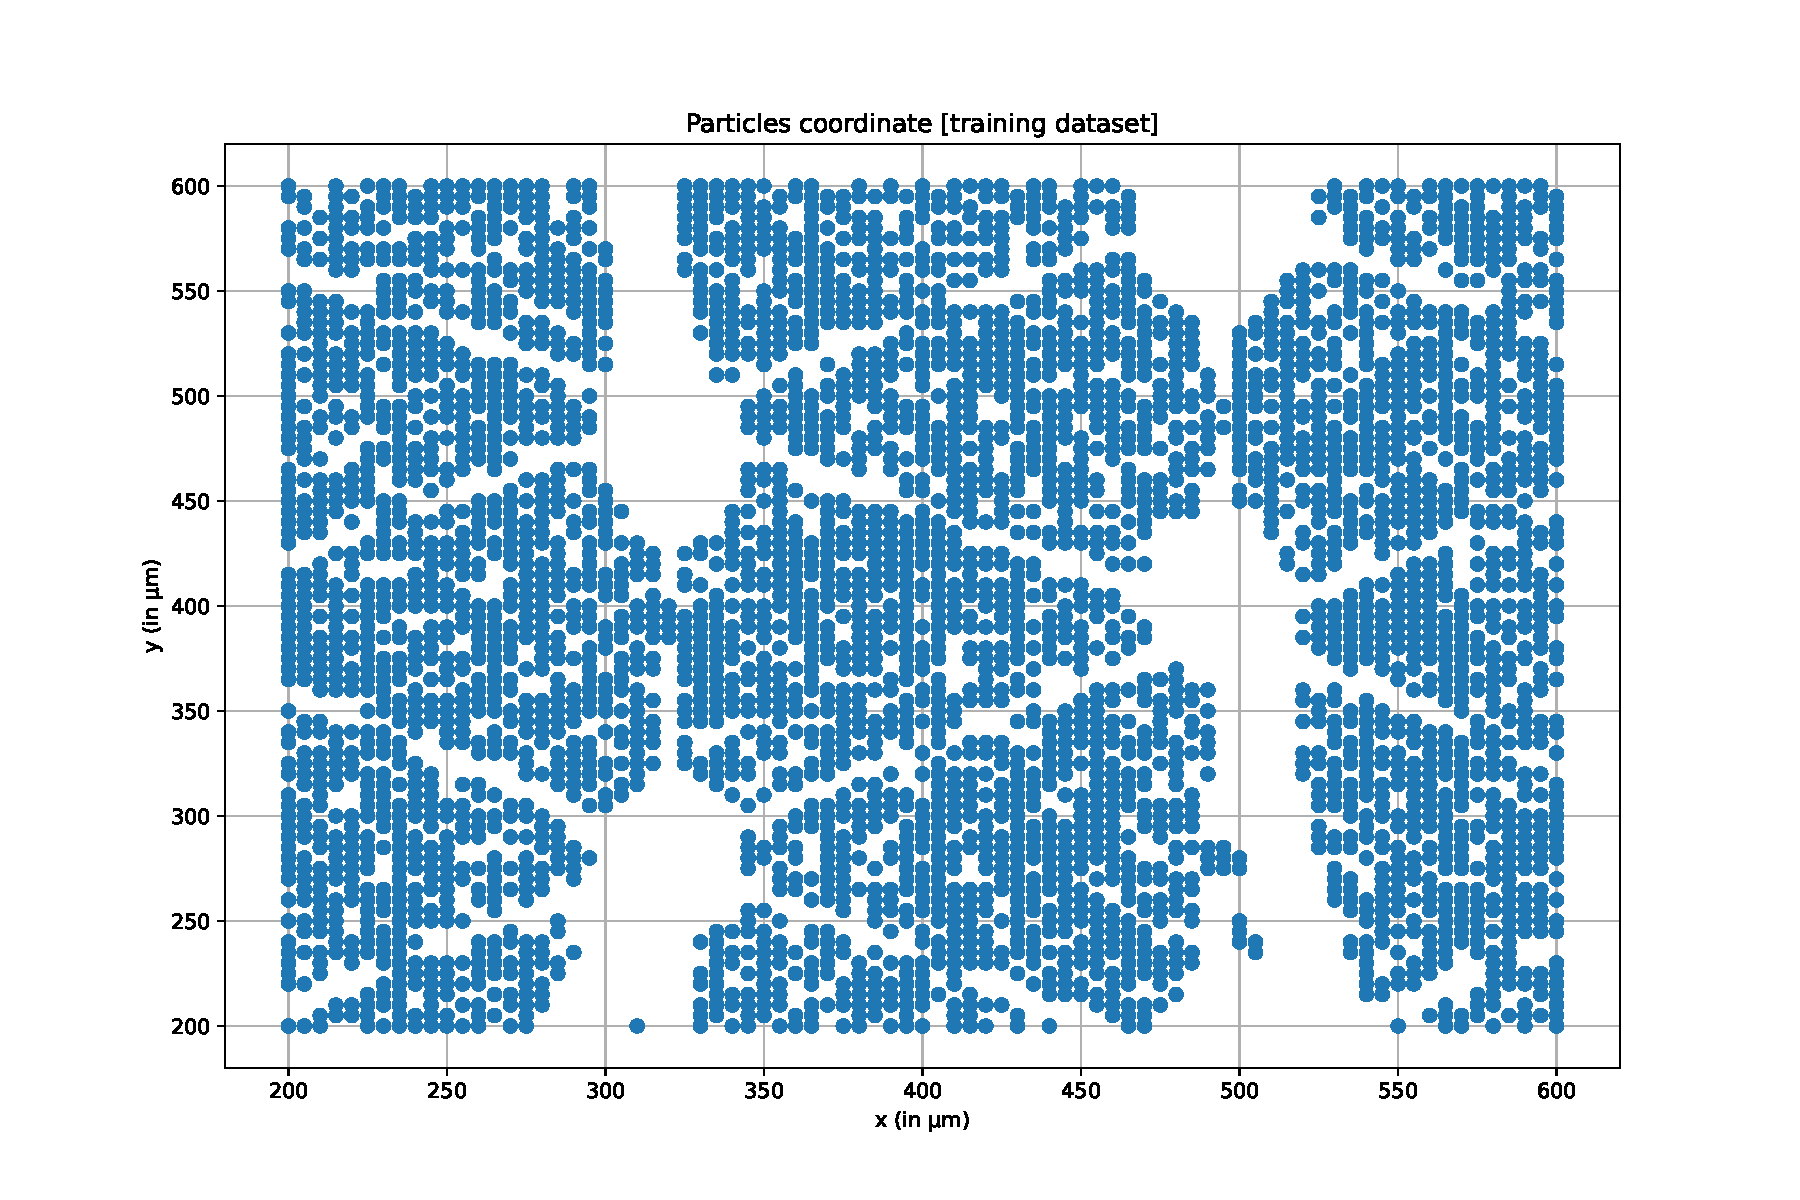
\includegraphics[width=\linewidth]{media/plot_dataset.png}}
\caption{Cartesian plane with the x and y coordinates.}
\label{fig:cartesian_plane}
\end{figure}

The preprocessing phase begins by understanding the utility of all the 5 features extracted 
from the signals exported by the pads.

Feature selection process was employed during the preprocessing phase. After experimenting with 
various feature combinations, it was determined that the model yielded better results when 
trained on a subset of features. \cite{OpenAI_ChatGPT_help_me_on_this}
Features associated with \textit{“tmax”} and \textit{“rms”} were identified as less impactful, 
prompting their removal from the dataset.
This first phase removes 36 columns from the dataset.\\

To mitigate the noise generated from 18 readings across 12 pads, different feature 
selection methods have been implemented and tried with the objective of excluding 
columns that contain features that are noise:

\begin{itemize}
    \item \textit{VarianceThreshold}: a feature selection method that removes features with low variance, 
    considering them less informative. It was used with \textit{thresholds} equal to 0.35.
    \item \textit{SelectKBest}: a feature selection approach that selects the top k features 
    based on a scoring function. 
    It was used with \textit{k} equals to 60. This method focuses on retaining the k 
    most informative features.
    \item \textit{SelectFwe}: (Select Family-Wise Error rate): a feature selection method 
    that controls the family-wise error rate to reduce the likelihood of false discoveries. 
    It was used with the \textit{scoring function} equivalent to \textit{f\_regression}, 
    which assesses the linear relationship between each feature and the target 
    variable. \cite{OpenAI_ChatGPT_help_me_on_this}
\end{itemize}

After experimenting these feature selections methods with different parameters the \textit{SelectFwe} method 
was chosen. This feature selection method led to the removal of another 9 columns.\\

After removing all the useless and/or noise features all the remaining columns have been transformed 
in the range 0 to 1, meaning that the minimum and maximum value of a feature is going to be 0 and 1. 
For doing that the \textit{MinMaxScaler} preprocessing function has been applied to the dataset.


\subsection{Model selection}
In this context of regression analysis, where the objective is to predict continuous numerical values 
a regressor model needs to be used. After performing different tests, the selected model is the 
\textit{Extra Trees Regressor} from scikit-learn's python library, but we also used the 
\textit{Random Forest Regressor} for performing tests on different hyperparameters.

The \textit{RandomForestRegressor} is an algorithm belonging to the family of decision tree methods. 
Comprising an ensemble of numerous decision trees, this model excels in capturing complex 
relationships within datasets, making it particularly well-suited for regression tasks. 
Each decision tree in the ensemble independently learns patterns from the data, and the 
final prediction is an average or a weighted sum of predictions 
from individual trees. \cite{OpenAI_ChatGPT_help_me_on_this}
The ensemble nature of the model provides inherent regularization, reducing the risk of
overfitting and enhancing generalization to new data.

The \textit{ExtraTreesRegressor} is an algorithm that creates multiple trees and 
employs random subsets of features for node splitting. However, it differs in 
two key aspects: it does not bootstrap observations 
(sampling without replacement), and nodes are split based on random splits among a random subset
of features at each node. This distinctive approach contributes to its effectiveness in 
capturing patterns within the dataset. \cite{stackexchange_438384}


\subsection{Hyperparameters tuning}
Fine-tuning the hyperparameters of the predictive model is a crucial step towards 
achieving optimal performance. In this phase, we systematically explore different 
combinations of hyperparameters to identify the configuration that yields the best 
results. 
Grid Search is employed to methodically search through a predefined grid of 
hyperparameter values. This exhaustive search allow to evaluate the model's performance 
across various parameter combinations.\\

The pipeline has been evaluated splitting the development dataset. 
Initially, a partition of 75\% for training and 25\% for testing resulted in 366,225 training 
instances and 19,275 testing instances. Subsequently, in preparation for the final submission, 
a more focused 95-5\% split was adopted to augment algorithm training. 
The decision to reduce the test set to 5\% occurred post-hyperparameter tuning, enabling the 
algorithm to benefit from an increased volume of training data. This strategic adjustment 
contributes to the robustness and efficacy of the trained model.

\begin{table}[htbp]
\centering
\begin{tabular}{|c|c|c|c|c|} \hline
time&  preprocessing&  criterion&  max\_features& score\\ \hline
1m 03s&  none&  squared\_error&  log2& 5.181\\ \hline
1m 10s&  none&  squared\_error&  sqrt& 4.703\\ \hline
1m 32s&  none&  friedman\_mse&  sqrt& 4.700\\ \hline
1m 49s&  note&  poisson&  sqrt& 4.695\\ \hline
6m 02s&  none&  squared\_error&  0.45& 4.251\\ \hline
8m 16s&  none&  squared\_error&  0.60& 4.286\\ \hline
4m 50s&  variance&  squared\_error&  0.45& 4.222\\ \hline
3m 37s&  SelectFwe&  squared\_error&  0.45& 4.171\\ \hline
2m 16s&  SelectFwe+FS&  squared\_error&  0.45& 4.154\\ \hline
\end{tabular}
\caption{Trying different hyperparameters and different preprocessing methods on RandomForestRegressor}
\label{tab:hyperparameters_table}
\end{table}

Table \ref{tab:hyperparameters_table} provides an overview of the time invested, 
preprocessing techniques applied, criterion selection, maximum features considered, 
and the local resulting scores achieved during the hyperparameter tuning process. 
It serves as a valuable reference to understand the evolution of our model's 
configuration and its corresponding impact on performance.

The \textit{RandomForestRegressor} was tested with various key hyperparameters. 
Additionally, the \textit{Number of Estimators}, which indicates the number
of decision trees in the ensemble, was a parameter of significant consideration.
The \textit{Number of Estimators} influence both execution time and model precision, 
prompting a meticulous examination. For our preliminary tests, we consistently set 
this parameter to 100 (the default value). 
However, for the final submission, we conducted tests with up to
400. This adjustment led to an increase in the model's fit time. 
However, an observation was the reduction in the \textit{Euclidean distance}
score, a positive outcome achieved without having overfitting problems.


\section{Results}
For the evaluation of the data science pipeline, we rely on two evaluation metrics:
\begin{itemize}
    \item \textit{R-squared} score \textit{(R²)}: serves as a pivotal measure to gauge the proportion 
    of variance in the target variable that our model explains. A \textit{R²} score near to 1 
    means a stronger correlation between predicted and actual values, indicative of 
    improved predictive accuracy.
    \item \textit{Euclidean distance} score: quantifies the spatial disparity between predicted and 
    actual particle positions, providing a more granular assessment of the model's 
    precision. \cite{OpenAI_ChatGPT_help_me_on_this}
    This score will be used for the project evaluation.\\
\end{itemize}

During the hyperparameter tuning phase, interpreting the \textit{R-squared} score was 
challenging as it consistently hovered around 0.99, reflecting a high level of correlation 
between predicted and actual values. Consequently, our focus shifted to the 
\textit{Euclidean distance} score, which provided a more readable assessment.

In the initial tests, the \textit{R²} score registered 0.99848024, while the \textit{Euclidean 
distance} stood at 5.181. Following hyperparameter tuning, these metrics further improved, 
reaching an \textit{R²} score of 0.99903096 and a reduced \textit{Euclidean distance} of 4.251.

Subsequently, preprocessing techniques were applied to refine the model's performance:
\begin{itemize}
    \item Using \textit{VarianceThreshold} the \textit{Euclidean distance} further decreased to 4.222.
    \item Using \textit{SelectFwe}: approach resulted in a \textit{Euclidean distance} of 4.171.
    \item \textit{SelectFwe} + Feature Selection removing redundant features such 
    as \textit{“tmax”} and \textit{“rms”} contributed to an 
    \textit{Euclidean distance} of 4.154.
\end{itemize}

These adjustments and preprocessing steps not only fine-tuned our model but also spotlighted 
the significance of carefully chosen evaluation metrics, ensuring a comprehensive understanding 
of the pipeline capabilities.\\

As outlined in the hyperparameters section, all these tests were conducted with 
the \textit{Number of Estimators} set to 100. In preparation for submission, the algorithm 
was refitted with 400 estimators, resulting in a \textit{Euclidean distance} 
of 3.907, obtained after 5 minutes of fitting. 
However, the score obtained with the submitted CSV file was 4.479. 
It is worth noting a consistent pattern where the submission platform tends to yield a 
score approximately 0.6 higher than the local score.

\begin{figure}[htbp]
\centerline{\includegraphics[width=\linewidth]{media/plot_prediction.png}}
\caption{Cartesian plane with prediction dataset.}
\label{fig:cartesian_plane_prediction}
\end{figure}

In Figure \ref{fig:cartesian_plane_prediction}, each event predicted by the pipeline
is collocated on a Cartesian plane using the predicted feature \textit{x} and \textit{y}.
This is a representation of the evaluation.csv submitted to the scoring platform.


\section{Discussion}
In this project paper, we have presented a viable solution for predicting the 
position of a particle based on a set of extracted features from signals obtained 
through sensor measurements.

In our exploration, we initially directed our attention to the \textit{RandomForestRegressor}, 
experimenting with various hyperparameters to fine-tune its performance. 
While these attempts yielded valuable insights, the pursuit of further improvements 
led us to test the \textit{RandomForestClassifier}. With this classifier the 
local \textit{Euclidean distance} score failed to reach the desired levels, peaking at 7.

\begin{figure}[htbp]
\centerline{\includegraphics[width=\linewidth]{media/plot_prediction_classifier.png}}
\caption{Cartesian plane with prediction dataset if using a classifier.}
\label{fig:cartesian_plane_prediction_classifier}
\end{figure}

Figure \ref{fig:cartesian_plane_prediction_classifier} provides a visual 
representation of the predicted \textit{x} and \textit{y} positions where the 
coordinates of all the predicted signals are grouped in different clusters.\\

We finally chose the \textit{ExtraTreesRegressor}, utilizing 
the same hyperparameters as the \textit{RandomForestRegressor}. Remarkably, this adjustment 
resulted in a significantly improved \textit{Euclidean distance} score, lowering to 3.907, with a 
fitting time of near 5 minutes. This effort produced a final score of \textbf{4.479}.\\

Examining the leaderboard, it becomes apparent that superior results have been achieved,
placing our solution in the top 22\%. While acknowledging that better solutions are 
available, we think that our achieved score is considered quite good. 
It is important to contextualize the significance of the score within the constraints
of the problem. Given that the sensor's \textit{x} and \textit{y}
measurements are multiples of 5, 
and our score is lower than 5, the margin of error falls within an acceptable range.\\\\


\bibliography{bibliography}
\bibliographystyle{ieeetr}

\end{document}
